\sect{Classical Robot Programming and Interaction Methods}{classicalprogramming}

Industrial robot programming has progressed from manual, vendor-specific procedures toward open and interoperable frameworks. Initially, robots were programmed using teach pendants that allow operators to define trajectories, waypoints, and parameters such as velocity and acceleration in a point-to-point manner, with all positions stored in the controller for playback \cite{teachpendant}. The approach is appreciated for its low cost, transparency, and direct feedback. Recent wireless versions increase operational safety by allowing use outside hazardous areas. However, it remains highly time-consuming and inflexible, since any change in the process requires full re-teaching of the sequence. Moreover, the absence of standardised interfaces across manufacturers limits reuse and scalability, prompting the transition toward virtual and software-based programming environments \cite{teachpendant}.


Parallel to teach pendants, proprietary robot programming languages such as KUKA Robot Language (KRL), ABB RAPID, and Fanuc TP became the dominant tools for defining motion commands, process logic, and I/O operations \cite{app13042582}. These languages ensure deterministic execution, safety, and integration with dedicated controllers. However, their vendor-specific syntax and structure hinder interoperability between robot brands, complicate multi-robot coordination, and limit accessibility for non-expert users. Updating or modifying a process typically requires stopping the robot and redeploying code, resulting in production downtime \cite{app13042582}. Table \ref{tab:vendor_lang} summarises the most common vendor-specific languages used in industrial practice.

\begin{table}[H]
\centering
\begin{tabular}{l|l}
\textbf{Manufacturer} & \textbf{Programming Language} \\ \hline
KUKA                & KRL (KUKA Robot Language)      \\
ABB                 & RAPID                          \\
FANUC               & TP (Teach Pendant Language)    \\
Yaskawa Motoman     & INFORM                         \\
Universal Robots    & URScript                       \\
Kawasaki Robotics   & AS Language                    \\

\end{tabular}
\caption{Examples of vendor-specific programming languages used in industrial robots.}
\label{tab:vendor_lang}
\end{table}

Offline Programming (OLP) and simulation environments were developed to address these limitations. They allow program generation and verification in a virtual workspace without occupying the physical robot, which significantly reduces downtime and enables preparation before installation \cite{SicilianoKhatib2008}. Contemporary OLP tools combine physics-based simulation and virtual controllers to validate trajectories, detect singularities, assess reachability, and perform collision and cycle-time analysis. Integration with CAD/CAM models enables direct path generation from geometric data and optimisation of robot configurations before deployment. Although OLP enhances efficiency and safety, its accuracy strongly depends on model fidelity and calibration quality, often necessitating final tuning on the real robot for sensor-based or tolerance-critical operations. Representative OLP systems include following examples in Table \ref{tab:olp_tools}.

\begin{table}[H]
\centering
\begin{tabular}{l|l}
\textbf{Software Tool} & \textbf{Vendor/Developer} \\ \hline
RobotStudio           & ABB                         \\
KUKA.Sim             & KUKA                        \\
RoboDK               & RoboDK                      \\
Process Simulate      & Siemens                     \\
PowerMill Robot       & Autodesk                    \\
\end{tabular}
\caption{Examples of offline programming and simulation tools.}
\label{tab:olp_tools}
\end{table}

The increasing complexity of multi-robot and sensor-integrated systems has accelerated the adoption of open-source middleware and API-based interaction frameworks \cite{quigley2009ros}. The Robot Operating System (ROS) introduced a distributed, message-oriented architecture built around topics, services, and actions. It supports multiple programming languages and enables modular software composition and reuse \cite{quigley2009ros}. ROS2 extended this paradigm by implementing DDS-based communication for real-time and deterministic performance, making it suitable for industrial-grade applications \cite{hiillos2023design}. Similarly, the Robotics API formalised a high-level abstraction for robot operations through commands, events, and triggers while delegating real-time execution to a control core \cite{angerer2010robotics}.

\begin{figure}[H]
\centering
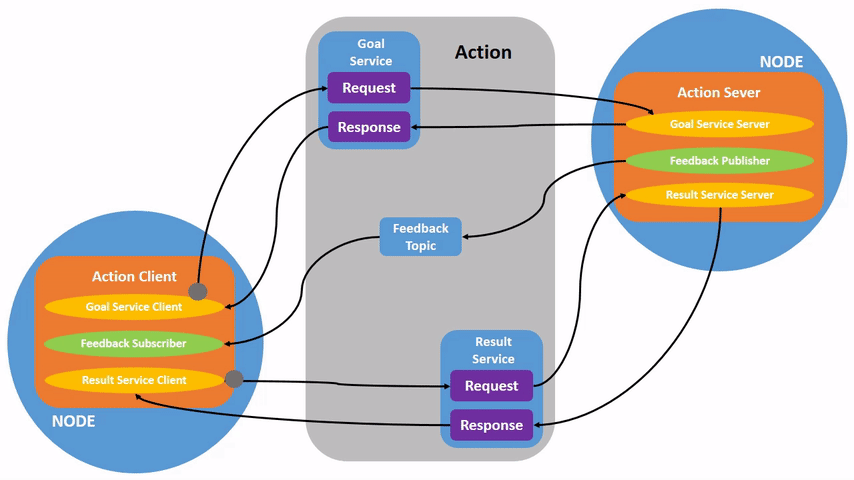
\includegraphics[width=1\linewidth]{Images/ros2action.png}
\caption{Structure of a graph-based interface in ROS2 \cite{rosUnderstandingActions}.}
\end{figure}

Middleware and API frameworks enable hardware-independent control through standardised interfaces and object-oriented data models. They facilitate interoperability among heterogeneous systems, support integration with sensors and cloud platforms, and accelerate prototyping through reusable components \cite{quigley2009ros, hiillos2023design}. Despite these benefits, open frameworks still face challenges related to real-time guarantees, cybersecurity, and version compatibility.

In summary, the evolution of classical robot programming reveals a clear trajectory from manual point-to-point teaching to model-based and modular software architectures. Teach pendants remain accessible yet inefficient, vendor-specific languages ensure reliability but limit interoperability, and OLP enhances productivity but requires high-precision calibration. Modern middleware and API-based systems achieve abstraction and composability but are still constrained by timing and security requirements. These limitations motivate current research efforts toward AI-driven programming, where reinforcement learning and intent recognition aim to automate skill acquisition and enable adaptive, human-aligned robot behavior.